\section{Design}
\begin{frame}{Fundamental Designs}
    \begin{block}{Monolithic}
        \begin{itemize}
            \item Small number of modules
            \item Complex functionality within a single module
            \item Avoiding compound modules
        \end{itemize}
    \end{block}
    \begin{block}{Modular}
        \begin{itemize}
            \item High number of modules
            \item Small functionality within a single module
            \item Combination of multiple modules to compound modules
        \end{itemize}
    \end{block}
\end{frame}

\begin{frame}{Performance Measurement}
    \begin{block}{Measurement Methods}
        \begin{description}[created events]
            \item[runtime] Measurement of the runtime required to simulate a given amount of simulation time
            \item[created events] Measurement Measurement of the number of created events withing a fixed runtime
            \item[real-time] Observation of the real-time simulation indicator (performance ratio) during a parameter sweep for the data generation interval
        \end{description}
    \end{block}
\end{frame}

\begin{frame}{Example Network}
    \begin{block}{Structure}
        \begin{multicols}{3}
            \begin{itemize}
                \item Generator
                \item Dispatcher
                \item Various sinks
            \end{itemize}
        \end{multicols}
    \end{block}
    
    \begin{figure}
        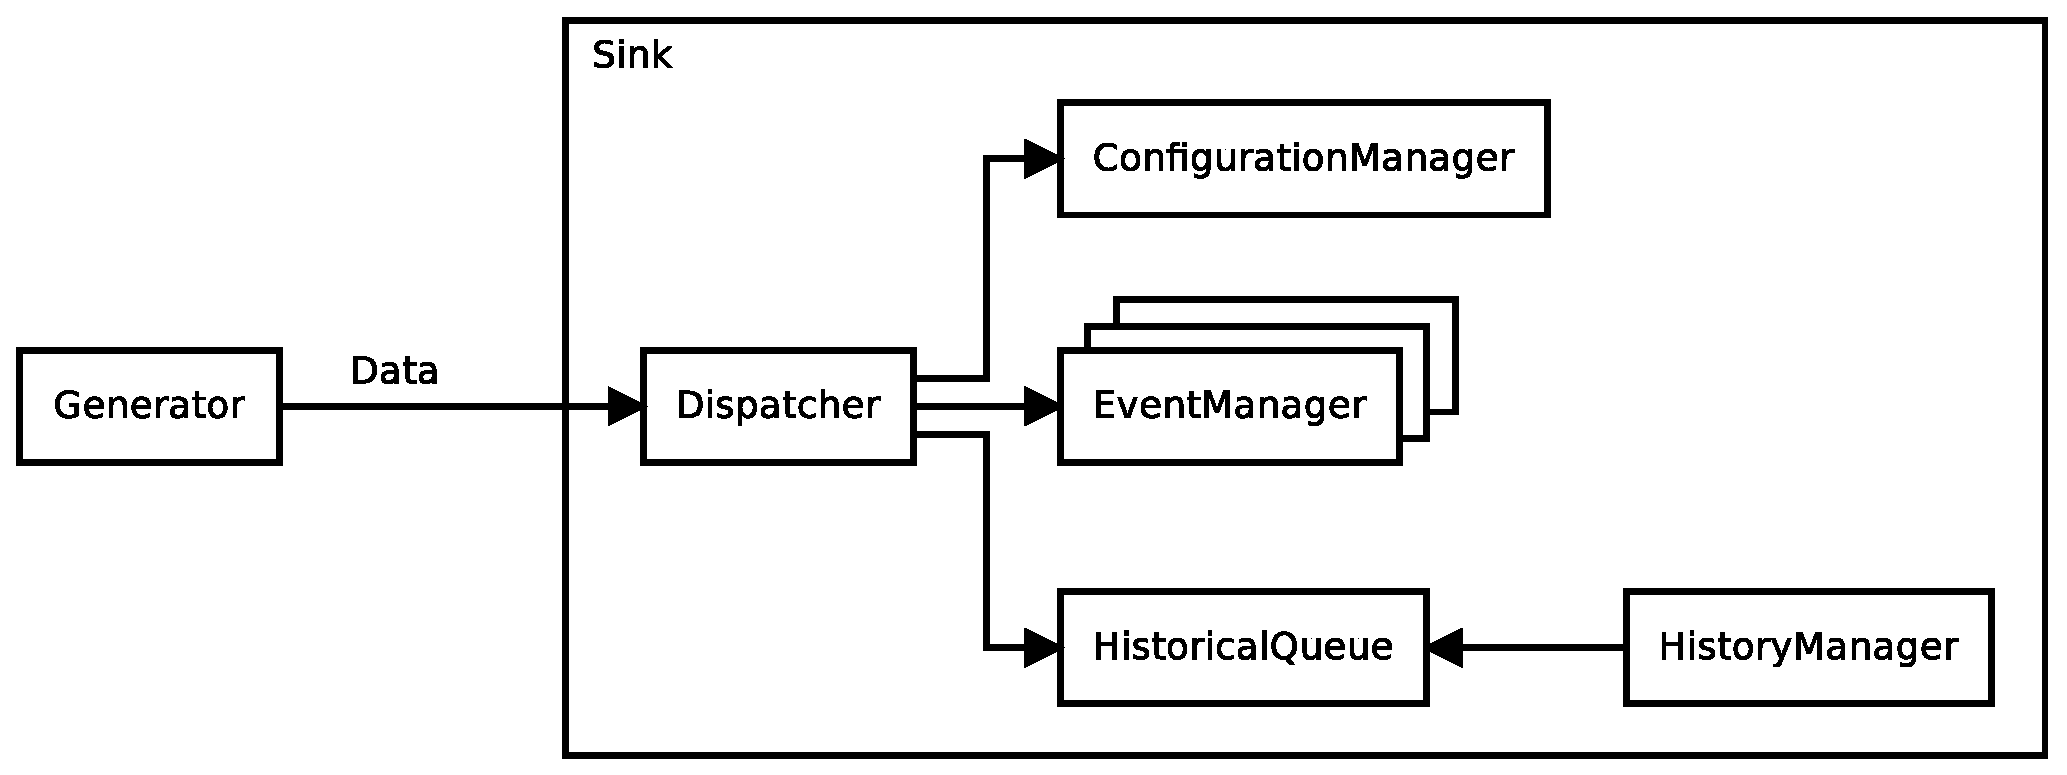
\includegraphics[width=0.9\textwidth]{../../thesis/images/design_test_network.eps}
    \end{figure}
\end{frame}

\begin{frame}{Results}
    The average ratio of performance values using a modular design over a monolithic design.
    \begin{columns}
        \begin{column}{0.48\textwidth}
            \begin{block}{Sequential\strut}
        \begin{description}[created events]
            \item[runtime] $4.033$
            \item[created events] $0.288$
            \item[real-time] $1.592$
        \end{description}
            \end{block}
        \end{column}
        \begin{column}{0.48\textwidth}
            \begin{block}{Parallel\strut} %TODO: eventually remove block
                \begin{description}[created events]
                    \item[runtime] 9999
                \end{description}
            \end{block}
        \end{column}
    \end{columns}
    
\end{frame}